\chapter{Descripción del Trabajo}
\label{cap:descripcionTrabajo}
\section{Diseño de la herramienta}
\label{sec:Descripción de la herramienta}
Se desea diseñar una herramienta donde dado el usuario unas imágenes, unas configuraciones y el texto esperado, el programa pueda reconocer el texto de la imagen y detectar si existe algún error de localización de las que hemos seleccionado.
La idea es que esta herramienta sea utilizado como ayuda al personal de LQA como parte del desarrollo del videojuego.
El usuario proporciona los datos necesarios para la ejecución de la herramienta, seguido la herramienta recoge los datos, estos datos son enviados al OCR para el reconocimiento de texto y otras informaciones relevantes (p.ej posición del texto), después, se envia toda la información a los tests para detectar la existencia de algún error y esto será enviado de nuevo al programa principal generando así un informe de los resultados.(Figura \ref{fig:Descripcion_Herramienta})
\begin{figure}[H]
	\centering
	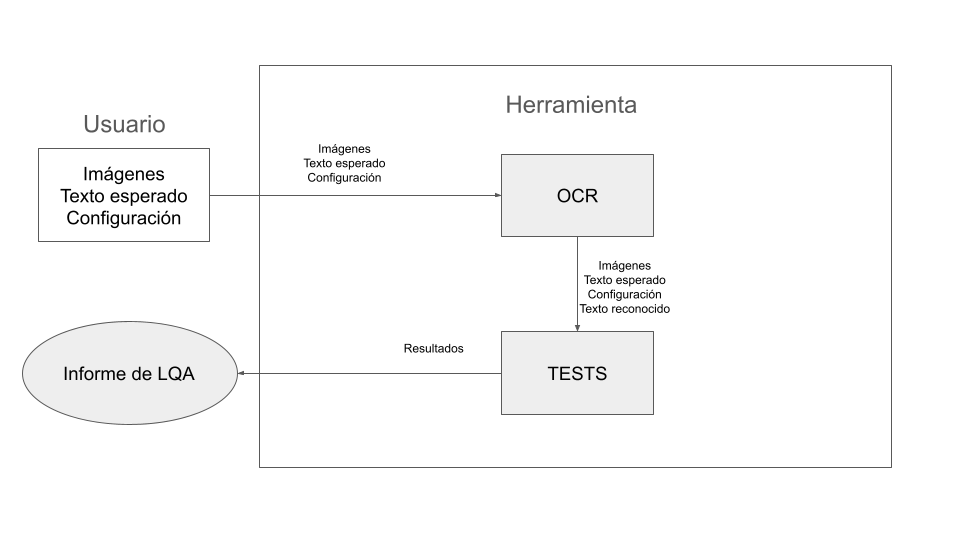
\includegraphics[width = 1\textwidth]{Imagenes/Descripcion_Herramienta.png}
	\caption{Dibujo con los módulos y la información que se pasa.}
	\label{fig:Descripcion_Herramienta}
\end{figure}

Para ello la herramienta además del programa principal, constará de dos módulos:
\begin{itemize}
	\item Modulo del OCR.
	\item Modulo del test.
\end{itemize}
\section{Modulo de OCR}
\label{sec:Modulo_OCR_Des}
El modulo de OCR se encarga de todo lo relacionado con la detección de texto en imágenes y la mejora de la detección.

En este modulo se elegirá una librería de OCR para la detección de texto y tendrá principalmente dos funcionalidades: 
\begin{itemize}
	\item Entrenar modelo: Dado una fuente y un idioma, el OCR entrena un modelo especifico para esa fuente en concreta y ese idioma en concreto, mejorando así el resultado obtenido. Este proceso se hace una sola vez como preparación previa de la herramienta, pero si el usuario desea o necesita varias fuentes o idiomas, puede generarlas las veces que sea necesario.
	\item Reconocer texto: Dado una imagen o una ruta de imagen, el OCR reconoce texto de todas la imágenes y los guarda en la ruta destino y se los pasa al programa. 
\end{itemize}
En este módulo, recibirá los datos proporcionado por el usuario y se procesará multiples imagenes con un modelo en concreto ya sea entrenado o el por defecto de la herramienta. En la configuración es necesario que el usuario proporcione información como:
\begin{itemize}
	\item La ruta de la imagen.
	\item La ruta del texto esperado.
	\item La ruta del modelo a utilizar.
	\item Nombre del modelo a utilizar.
\end{itemize}
Con las imágenes, pasará por un proceso de preprocesado para mejorar la calidad de la imagen en el sentido de que el OCR reconozca mejor los caractéres y generará un texto.
Ese texto antes de ser pasado como entrada al siguiente modulo será procesado otra vez para minimizar el error producido por el OCR.
Debido a la necesidad de algunos test, también se ha considerado obtener informaciones como posición del texto en la imagen en este modulo.
\section{Modulo de test}
El modulo de test se cargará de verificar si existe algún error de localización con el texto obtenido del OCR.

Usará como entrada el texto reconocido del modulo de OCR y el texto esperado, proporcionado para validar los tests. Pasará por una serie de tests para verificar si existe o no algún error de localización. La salida de este modulo será el resultado de los tests indicando si ha pasado el tests y en caso negativo indicar (si es posible) donde se produce el fallo.

Con esa salida se generará un archivo con la información de los resultados que luego será interpretado para que sea entendible por un ser humano.

No se va a atacar todos los tests de descritos en la sección \ref{sec:Errores de localizacion}. 
Se elegirá unos de los tests de todos los errores comunes de localización y como se atacará ese error. Se ha elegido estos errores considerando la importancia y la relevancia con nuestra herramienta(p.ej atacar el error de audio no tiene sentido en este trabajo).
\subsection{Similitud}
\label{test:Simi}
Este es el test ``master'', la cual es ejecutado antes de todos los tests que viene a continuación. Su principal funcionalidad es para obviar la ejecución de algunos tests y mejorar el rendimiento del programa obviando ejecuciones innecesarias. En este test se obtiene la cadena reconocida por el OCR y lo compara con la cadena esperada obteniendo un porcentaje de similitud. Si ambas cadenas son iguales, significa que no existe errores en cuanto al contenido del texto, por lo que se puede obviar algunos test como el de truncamiento(subsección \ref{test:trunc}) y el de placeholder(subsección \ref{test:placeholder}). Tests como el de solapamiento(subsección \ref{test:overlap}), no tiene que ver con el contenido del texto, sino de la posición, estas se siguen ejecutandose con normalidad.

\subsection{Solapamiento de texto}
\label{test:overlap}
Para resolver este problema se plantea usar el OCR para detectar las posiciones de los textos, seguido de una librería gráfica para detectar el contorno de la caja delimitadora guardado para ese texto, y obtener así sus posiciones. Comparando la posición del texto y la posición de la caja delimitadora obtenemos si el texto se está saliendo de la caja o no.

Para simplificar el test, damos algunas restricciones: 
\begin{itemize}
	\item En la imagen, el texto tiene que aparecer completamente en horizontal sin ninguna rotación sobre el eje X.
	\item Detectamos texto que sobresale por los lados.
	\item Tiene que estar resaltado y tener un claro contraste con el fondo y el texto para facilitar la detección.
	\item Debe tener una forma de caja o ventana(cuadriculada, cuadriculada redondeada). No sirve, por ejemplo, un bocadillo en forma de nube.
\end{itemize} 
La salida indicará si existe o no solapamiento en la imagen.

\subsection{Implementación Incorrecta}
\label{test:placeholder}
Este error aparece cuando por algún error del desarrollador aparecen placeholders en la pantalla del juego en vez del texto(p.ej si en el juego me llamo ``pepe'', en vez de aparecer en el dialogo ``Hola pepe'', aparece un ``Hola      \texttt{\%*player\_name*\%''}).
Para resolver este problema es necesario especificar como entrada cuál es el formato utilizado para el placeholder indicando su apertura y cierre. Con los datos, hacer una búsqueda del placeholder en el texto reconocido por el OCR.

Se tiene en cuenta las siguientes restrincciones:
\begin{itemize}
	\item El placeholder es formado por al menos un carácter de apertura y al menos un carácter de cierre. Puede tener más de un carácter en ambos lados.
	\item Todo lo que este entre la cadena de apertura y cadena de cierre se considera placeholder sin importar el número de palabras que hay dentro.
	\item Existe un solo tipo de placeholder, de momento no soporta la detección de múltiples tipos de placeholders.
\end{itemize}
La salida indicará si existe placeholder en la imagen y la posición en la que se encuentra para una mejor búsqueda por parte del personal de QA.
\subsection{Truncamiento de texto}
\label{test:trunc}
Para resolver este problema se plantea obtener la cadena esperada y la cadena reconocida por el OCR. Se compara la longitud de ambas cadenas, si la longitud es la misma, entonces no existe truncamiento. En caso contrario, se hará comparaciones palabra a palabra buscando la existencia de subcadenas (p.ej ``ment'' es subcadena de ``mente''), en caso de encontrar subcadenas, entonces existe un truncamiento. Si no se encuentran subcadenas, significa que son diferentes frases por lo que sería otro tipo de error.

La salida indicara si existe o no truncamiento en el texto.

\section{Informe de resultados}
Se ejecutarán todos los test sobre cada imagen, generando así un informe con los resultados donde tendrá:
\begin{enumerate}
	\item Nombre de la imagen.
	\item Texto esperado y texto reconocido.
	\item Pass/fail de los tests y información extra de los tests dependiendo de cada test.
\end{enumerate}
Con este informe se generará un html con la información de los resultados como se muestra en la figura \ref{fig:Descripcion_Informe}.
\begin{figure}[H]
	\centering
	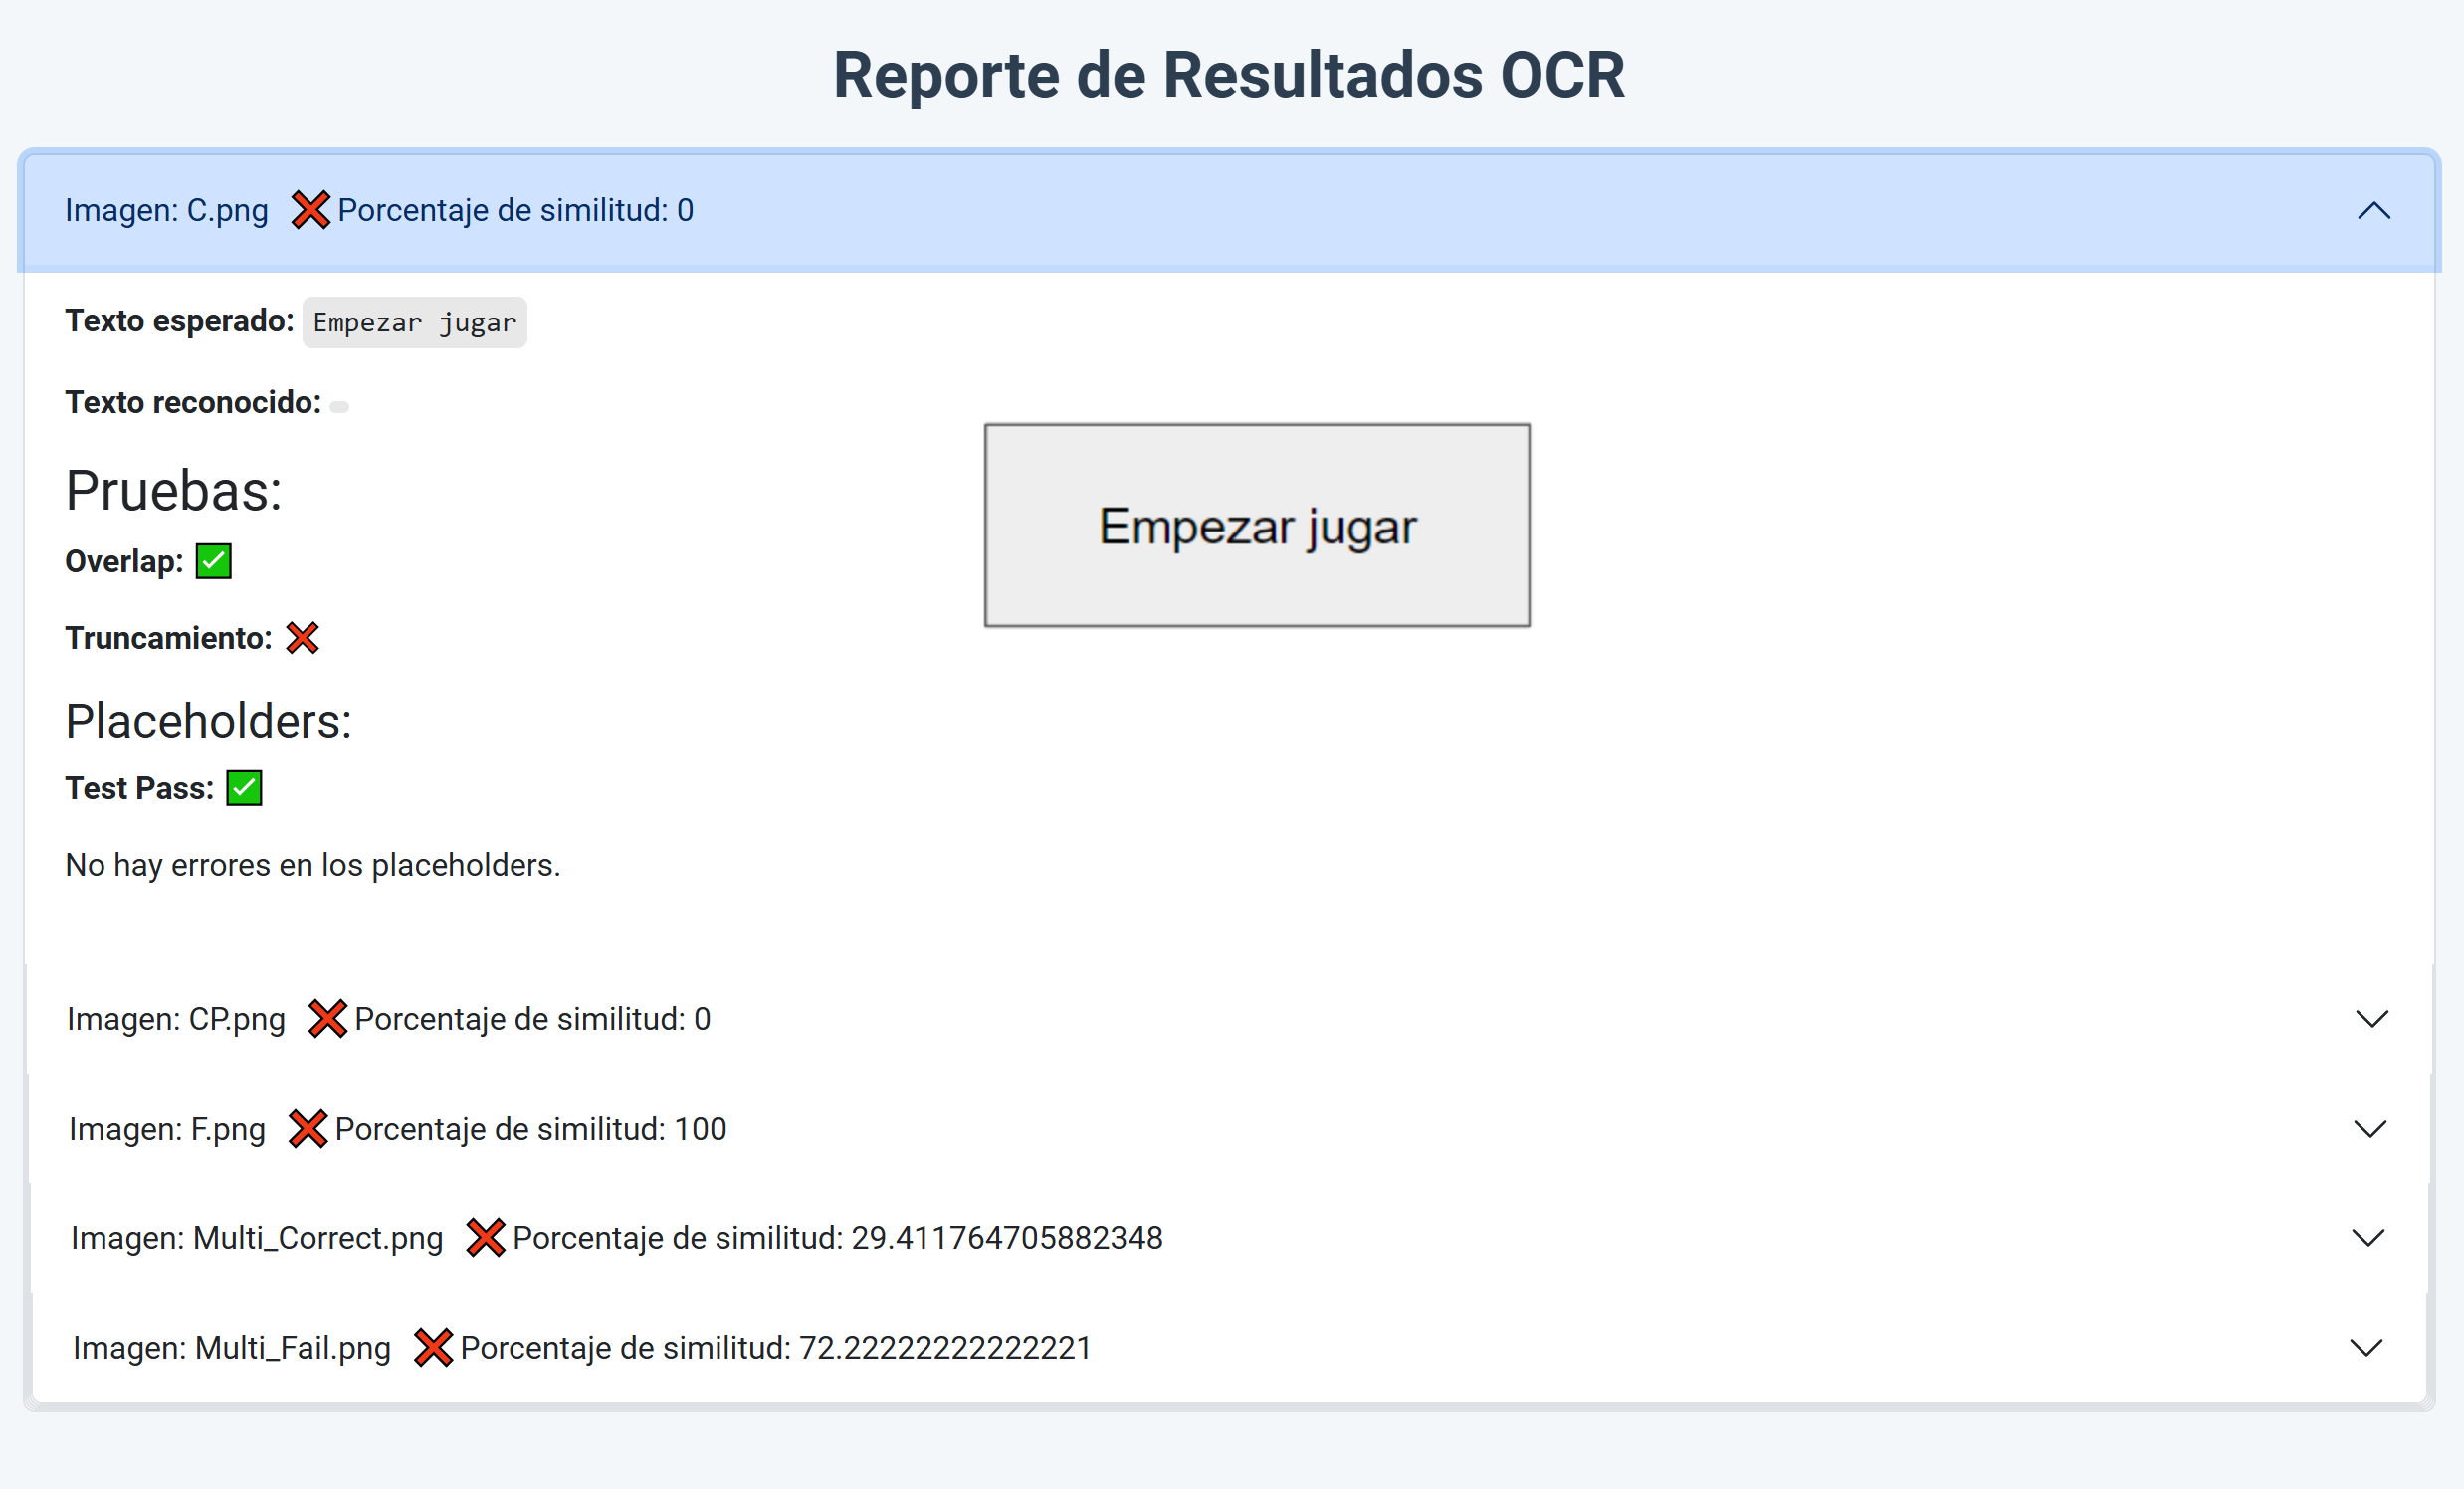
\includegraphics[width = 1\textwidth]{Imagenes/Des_Informe.png}
	\caption{Ejemplo de informe.}
	\label{fig:Descripcion_Informe}
\end{figure}
\section{Conclusión}
En este capítulo se ha descrito las partes de la herramienta detallando cada módulo, una para el reconocimiento de texto en imágenes usando OCR y otra para la comprobación de errores de localización usando tests. Donde el modulo de OCR recibirá como entrada las imágenes y una determinada configuración, reconocerá el texto y esta será pasado al modulo de tests para comprobar si existe algún error generando así un informe.
Una vez realizado el diseño de la herramienta, pasamos a describir como ha sido implementada en el siguiente capítulo.
 

